\documentclass[11pt,openany]{memoir}
\usepackage[usenames,dvipsnames]{xcolor}
\usepackage{amssymb}
\usepackage{amsmath}
\usepackage{amsthm}
\usepackage{url}
\usepackage{xspace}
\usepackage[margin=2.5cm]{geometry}
%\usepackage{tikz}
%\usetikzlibrary{positioning,calc,matrix,arrows}
%\usepackage{pgfplots}
\usepackage{listings}
\usepackage{color}
\usepackage{textcomp}
\usepackage{graphicx}
\usepackage{fancyvrb}
\usepackage{array}
\usepackage{dirtytalk}
\usepackage[colorlinks]{hyperref}
\usepackage{cleveref}

% NOTE: This template is based on the MatConvNet manual written by Andrea Vedaldi, Karel Lenc and Ankush Gupta.

\newtheorem{example}{Example}
\newtheorem{lemma}{Lemma}

\newcommand{\real}{\mathbb{R}}
\newcommand{\bx}{\mathbf{x}}
\newcommand{\bh}{\mathbf{h}}
\newcommand{\bw}{\mathbf{w}}
\newcommand{\by}{\mathbf{y}}
\newcommand{\bu}{\mathbf{u}}
\newcommand{\bv}{\mathbf{v}}
\newcommand{\pp}{\mathbf{p}}
\newcommand{\hh}{\mathbf{h}}
\newcommand{\XX}{\mathcal{X}}
\newcommand{\diag}{\operatorname{diag}}
\newcommand{\bone}{\mathbf{1}}
\newcommand{\FF}{\mathcal{F}}
\newcommand{\ththeta}{\pmb{\theta}}
\newcommand{\EE}{\mathbb{E}}
\DeclareMathOperator{\dd}{\text{d}}
\newcommand{\vv}{\operatorname{vec}}
\newcommand{\tr}{\operatorname{tr}}
%\newcommand{\matconvnet}{\textsc{MatConvNet}\xspace}
%\newcommand{\matlab}{\textsc{MATLAB}\xspace}
%\newcommand{\cpp}{C{}\texttt{++}~}
%\newcommand{\by}{\mathbf{y}}
%\newcommand{\bc}{\mathbf{c}}
%\newcommand{\bz}{\mathbf{z}}
%\newcommand{\bff}{\mathbf{f}}
%\newcommand{\bg}{\mathbf{g}}
%\newcommand{\br}{\mathbf{r}}
%\newcommand{\bw}{\mathbf{w}}
%\newcommand{\bp}{\mathbf{p}}
%\newcommand{\bfs}{\mathbf{s}}
%\newcommand{\bfe}{\mathbf{e}}
\newcommand{\samsays}[1]{\textcolor{RubineRed}{[S: #1]}}

\theoremstyle{plain}
\newtheorem{thm}{Theorem}[chapter] % reset theorem numbering for each chapter

\theoremstyle{definition}
\newtheorem{defn}[thm]{Definition} % definition numbers are dependent on theorem numbers
\newtheorem{exmp}[thm]{Example} % same for example numbers

%\newcommand{\argmin}{\operatornamewithlimits{argmin}}
%\newcommand{\argmax}{\operatornamewithlimits{argmax}}
%\newcommand{\sign}{\operatornamewithlimits{sign}}
%
%\tikzstyle{block} = [draw, rectangle, minimum height=3em, minimum width=3em]
%\tikzstyle{data} = []
%\tikzstyle{datac} = [draw, circle, minimum height=2.5em, minimum width=2.5em,inner sep=3pt,font=\footnotesize]
%\tikzstyle{par} = [draw, circle, minimum height=2.5em, minimum width=2.5em,fill=black!20,inner sep=3pt,font=\footnotesize]
%\tikzstyle{pinstyle} = [pin edge={to-,thin,black}]
%\tikzstyle{to} = [->,>=stealth',shorten >=1pt,semithick]
%\tikzstyle{from} = [<-,>=stealth',shorten >=1pt,semithick]
%\tikzstyle{bp} = [draw=blue,text=blue]
%\tikzstyle{bpl} = [draw=blue!40]
%\tikzstyle{bpe} = [text=blue,draw=none]

\VerbatimFootnotes

\setsecnumdepth{subsection}
\settocdepth{subsection}

\definecolor{listinggray}{gray}{0.9}
\definecolor{lbcolor}{rgb}{0.8,0.8,0.8}
\lstset{
	%backgroundcolor=\color{lbcolor},
	tabsize=4,
	%rulecolor=,
	language=matlab,
	basicstyle=\small,
	%upquote=true,
	%columns=fullflexible,
	%showstringspaces=false,
	extendedchars=true,
	%breaklines=false,
	%prebreak = \raisebox{0ex}[0ex][0ex]{\ensuremath{\hookleftarrow}},
	%frame=single,
	%showtabs=false,
	%showspaces=false,
	%showstringspaces=false,
	%identifierstyle=\ttfamily,
	keywordstyle=\color[rgb]{0,0,1},
	commentstyle=\itshape\color[rgb]{0.133,0.545,0.133},
	stringstyle=\color[rgb]{0.627,0.126,0.941},
}
%\lstMakeShortInline[columns=fullflexible, breaklines = true,
% breakatwhitespace = true]!

\title{Old Ideas for Applied Computer Vision}
\author{
Samuel Albanie
}
\date{}

% REMOVE TO FIX COMPILATION
\hypersetup{
  pdfinfo={
    Title={Classics/Kernels for Applied Computer Vision},
    Author={Samuel Albanie},
        Subject={Notes on Mathematics},
    Keywords={computer vision, differentials, machine learning}
  }
}

\sloppy

% ------------------------------------------------------------------
\begin{document}
% ------------------------------------------------------------------

%\end{document}

\frontmatter
\maketitle{}

\begin{abstract}
This note is designed to gather together information about some of the work that has gone on over the last few decades of computer vision research.
The goal is to develop it over time and therefore it should be considered a work-in-progress.  Consequently any contributions, feedback or notifications of mistakes are much appreciated\footnote{Feel free to contact me by raising an issue on the github page, submitting a pull request directly (\mbox{\url{https://github.com/albanie/derivations})}}).
\end{abstract}
\clearpage

\tableofcontents*
\clearpage

\mainmatter
\chapter{Introduction}\label{sec:intro}

Calculus plays a central role in computer vision. As the community has integrated ever more closely with techniques from machine learning, statistics and optimisation, the ability to differentiate vector and matrix functions has become more useful to computer vision researchers.  Unfortunately, multivariate calculus, when performed with indices over element locations is a fairly tricky business to build an intuition for.  Although the index-based approach has the majority of the market share in the research world, there is an alternative: the slightly lesser known method of \textit{matrix differentials}.  We have found this alternative approach to be significantly simpler, more intuitive and faster to work with.  

Finally, we note that the widespread adoption of automatic differentiation (autodiff) has been a major boon to the whole community, in many cases obviating the need to perform arduous pen and paper derivations.  The goal of these notes is not to encourage the reader to avoid using autodiff, but to assist them in understanding, on a mathematical level, what is going on \say{under the hood}.


\section{Useful Resources}

There are a number of extremely good references for getting to grips with the calculus of vector and matrix functions.  Below are a few that we have found particularly useful, providing much of the material for these notes:

\begin{itemize}
\item Written by econometricians Magnus and Neudecker (originally in $1988$, but revised several times), \textit{Matrix differential calculus with applications in statistics and econometrics} is the canonical reference for matrix differential calculus~\cite{magnus1988matrix}.
\item The fundamentals of working with matrices \cite{searle2017matrix}.
\item \cite{kinghorn1996integrals}, \cite{minka2000old} and \cite{petersen2008matrix} each contain a large number of highly useful results and are good as quick references.
\item The MatConvNet manual \cite{vedaldi2015matconvnetmanual} provides carefully worked through examples of matrix derivatives.  While the emphasis is primarily on index-based derivations, it provides the derivatives of many common neural network computation blocks in matrix form and is very useful as a reference. 
\end{itemize}
\chapter{Scale Space} \label{chap:scale-space}

One of the fundamental challenges in building systems that can understand images is the construction of good \textit{representations}.  Since even a relatively small image comprises a vast quantity of data, we would like to distill the information down to a much more compact form that tells us about the things we care about in the image and is \textit{invariant} to things we don't care about.  

Early work focused on simple representations of an image, such as the extrema in the signal (e.g. edges, dots etc.) and their first or second derivatives - a line sketch can contain much of the semantic content of an image while requiring far fewer bits of information to store.  However, this approach quickly runs into difficulties.  Over what scale should the derivatives of the image signal be taken?  Edges which define important for objects at one scale, such as the grains on a piece of wood, are irrelevant at another scale, such as a picture of a forrest. 

There have been several major contributions in this area, but perhaps the most important was the introduction of \textit{scale space filtering} \cite{witkin1987scale}.  The core idea is that the image should be represented simultaneously by a set of multiple scales.  This is achieved by simply convolving the source image with Gaussian filters of increasing bandwidth (this is illustrated with a one dimensional signal in Fig.~\ref{fig:scales}).  

\begin{figure}
\centering
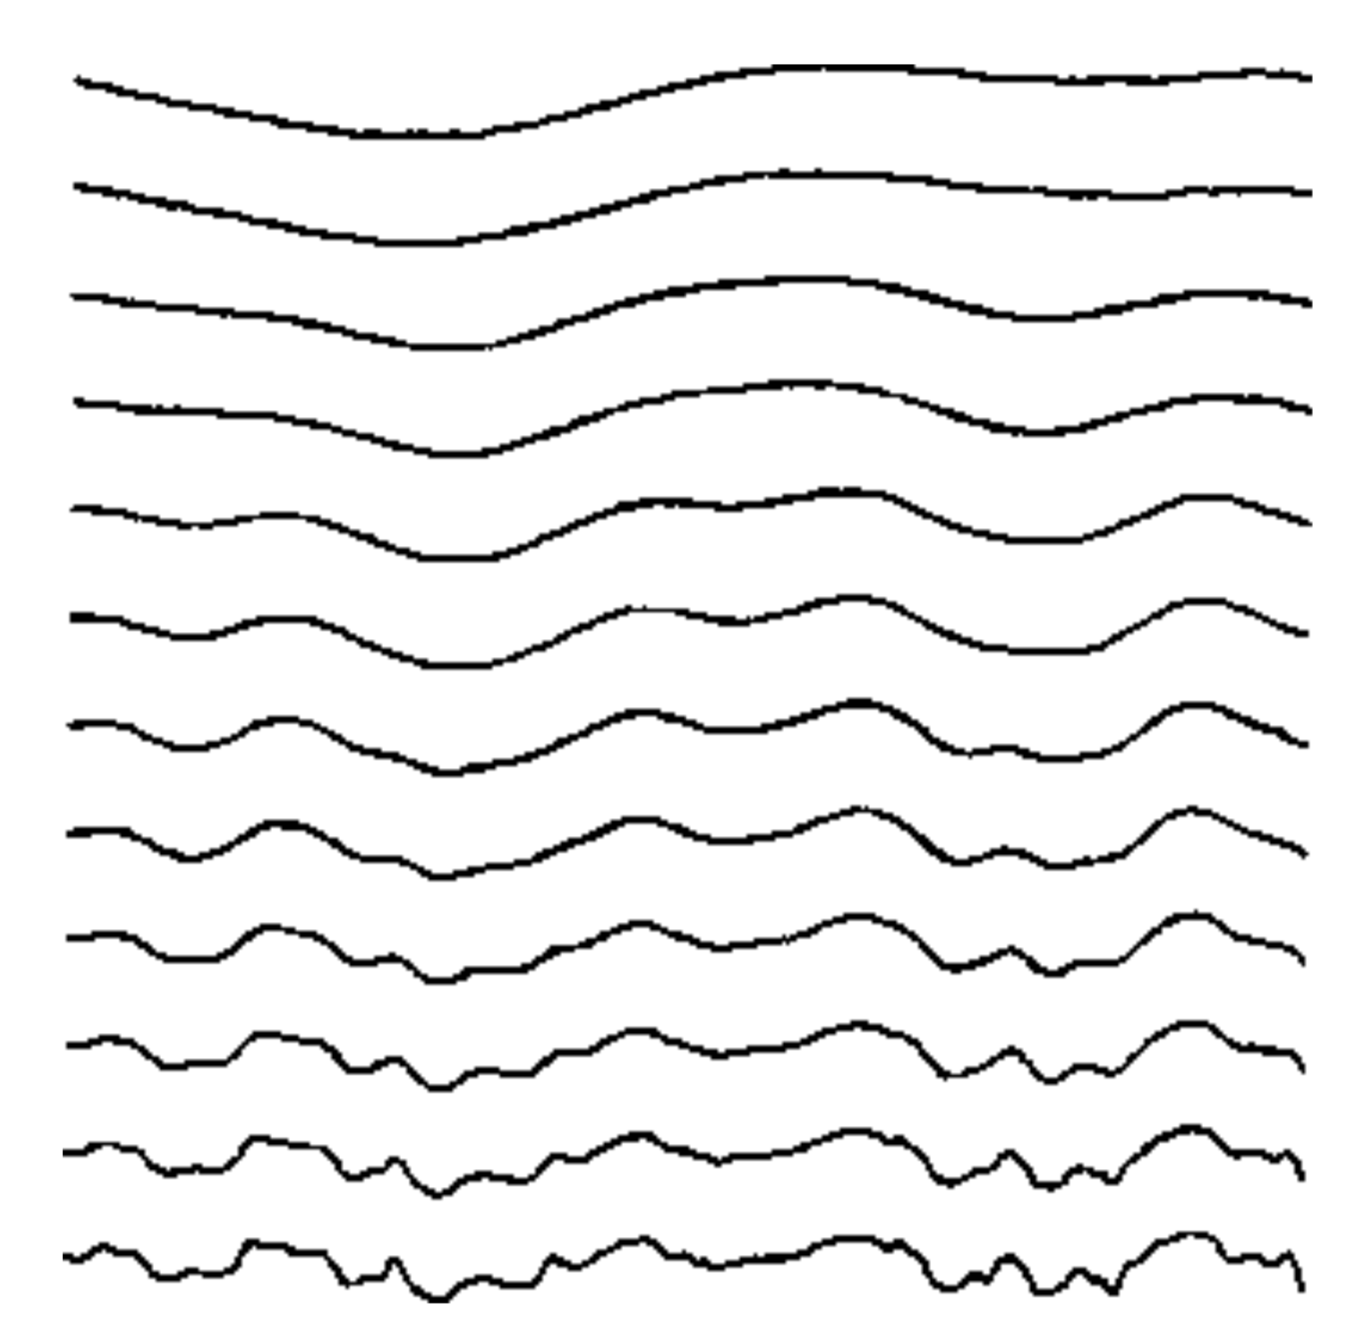
\includegraphics[height=0.3\textwidth]{figs/scale-space.png}
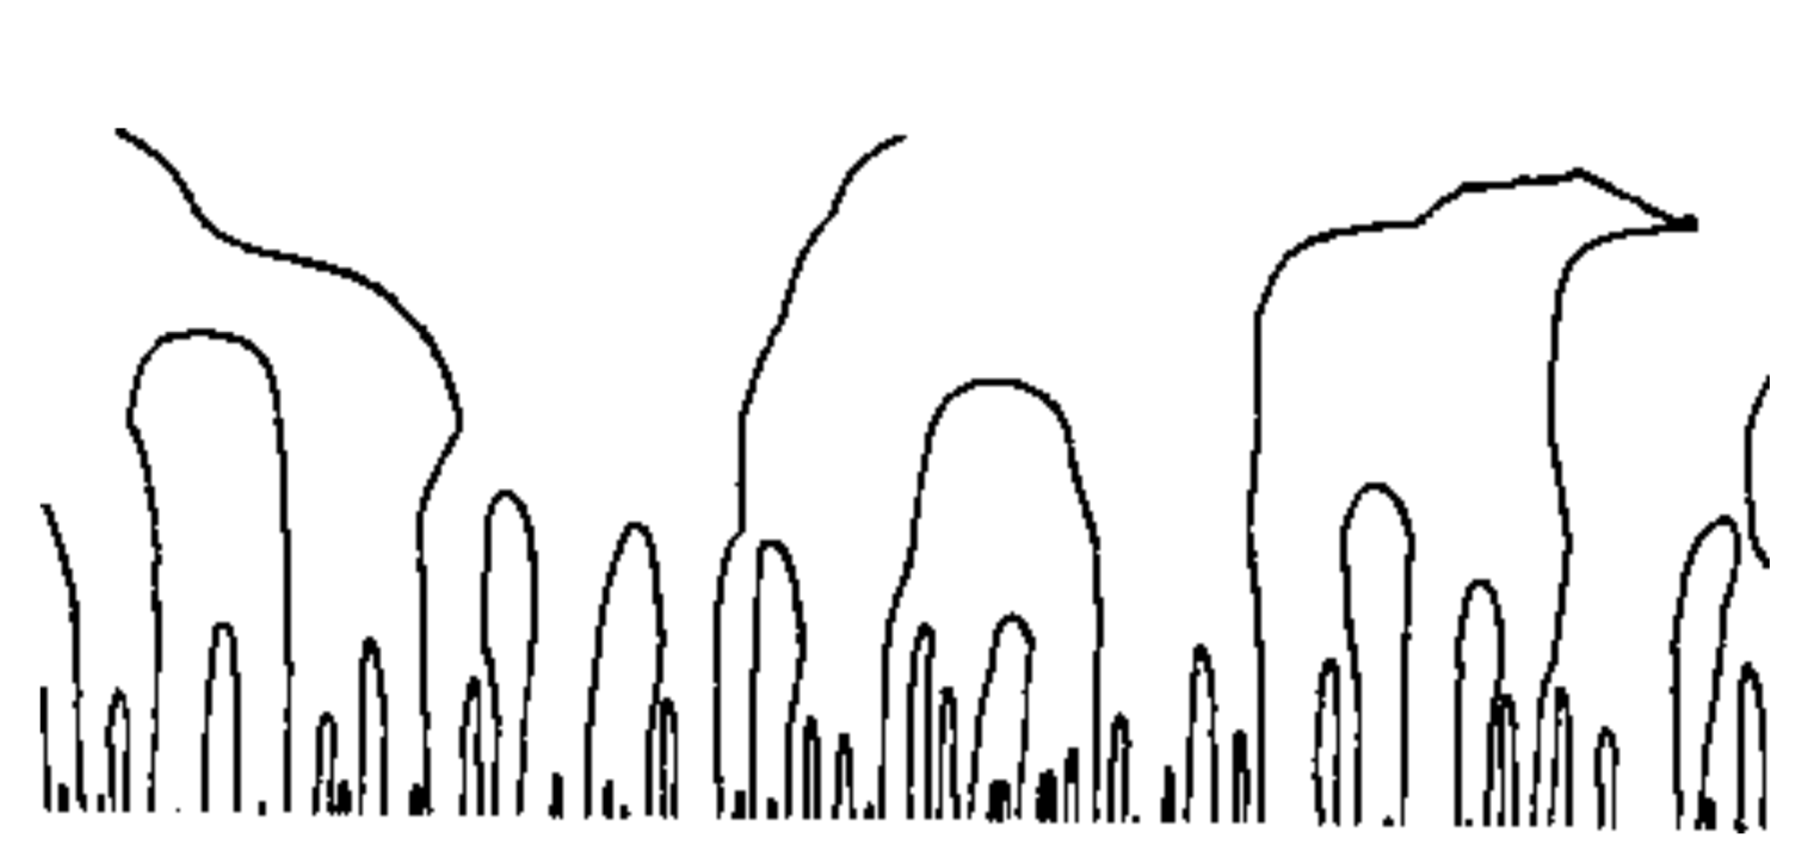
\includegraphics[height=0.25\textwidth]{figs/zero-crossings.png}
\caption{\textbf{Left}: The scale space of a one-dimensional signal $\phi$.  At the bottom is the raw signal, which has been smoothed by Gaussian kernels with increasing bandwidth as you move up the figure. \textbf{Right:} The level sets $ \phi_{xx} = $ corresponding to the scale space shown on the left.  In both images the $x$-axis is horizontal and the vertical axis represents the value fo $\sigma$ (the bandwidth of the smoothing kernel). These figures originally appeared in \cite{witkin1987scale}).\label{fig:scales}}
\end{figure}

In the original work, Witkin focused on using the zeros of the second derivative (i.e. the inflection points) of the signal as the representation

\appendix

\chapter{Functional Analysis for Kernels} \label{sec:functional-analysis}

This section builds up from basic definitions in functional analysis up to one of the key results (from a computer vision perspective) in this field of mathematics: the equivalence of kernels and inner products between feature maps.   In many cases it is sufficient to just be aware of this result at an intuitive level, without going through the details.  However, since a number of the papers that use kernels in computer vision require some knowledge of functional analysis (using the terminology of Banach spaces, RKHS etc.), having a grasp of the fundamentals can be helpful.  

These notes are based primarily on the material in \cite{sejdinovic2012rkhs}, with additional expansions where noted.  Following \cite{sejdinovic2012rkhs}, all the derivations will assume that vector spaces are defined over $\real$, but can be extended to other fields such as $\mathbb{C}$ if needed.

\section{Banach Spaces}

A Banach space is a vector space with certain topological properties. To describe these properties, we require a way to measure distances between elements in the space, which is provided by a \textit{norm}:

\begin{defn}
Let $\XX$ be a vector space.  Then $|| \cdot ||_{\XX} : \XX \rightarrow [0,\infty)$ is a called norm on $\XX$ if:
\begin{enumerate}
\item $|| \bx ||_{\XX} \geq 0 ,  \forall \bx \in \XX$ and $|| \bx ||_{\XX} = 0  \iff \bx = \mathbf{0}$ (the norm \textit{separates points})
\item $|| \alpha \bx ||_{\XX} = | \alpha | || \bx ||_{\XX} ,  \forall \bx \in \XX, \forall \alpha \in \real$ (homogeneity)
\item $ || \bx + \by ||_{\XX} \leq || \bx ||_{\XX} + || \by ||_{\XX}, \forall \bx, \by \in \XX$ (the triangle-inequality)
\end{enumerate}
\end{defn}

We can now measure distances between two elements of the space using a metric ${\dd}: \XX \times \XX \to \real$, defined using the norm as follows: ${\dd}(\bx, \by) = || \bx - \by ||_{\XX}$.

\begin{defn}
We say that a sequence $\{\bx_n\} \subset \XX$ converges to $\bx \in \XX$ if $\forall \epsilon > 0, \exists N \in \mathbb{N}$ such that $|| \bx_m - \bx ||_{\XX} < \epsilon, \forall m > N$.
\end{defn}



\chapter{Support Vector Machines} \label{sec:svms}

Support Vector Machines (SVMs) formed one of the dominant machine learning classification approaches in computer vision for a sustained period of time (late 90s to early 2010s onwards).  They are still widely used for a number of problems (although they often no longer represent the state-of-the-art in cases where large quantities of training data are available).  The overview here is based on the course notes by Andrew Ng \cite{svmsNg}.

The basic ideas of SVMs are easiest to understand in the context of binary classification (although they can be extended to more complex outputs with \textit{structural svms}).   We assume we are given a set of samples $\{\bx_i, y_i\}_{i=1}^n, \bx_i \in \real^d, y_i \in \{-1, 1\}$ drawn i.i.d. from the joint distribution $p(\bx,y)$.  We proceed to learn a model through risk minimisation \cite{vapnik1992principles}, which is to say that we aim to construct a model $f(\bx)$ that minimises the \textit{risk} of $f$ under this distribution:

\begin{align}
R(f) = \EE[l(f(\bx, \bw), y)] \label{eqn:risk}
\end{align}

where $\bw$ represent the parameters of the function. In practice, we cannot compute the expectation in Eqn.~\ref{eqn:risk} because we do not have access to the full underlying joint distribution $p(\bx, y)$.  However, since we have assumed that we have access to a handful of samples, we can approximate this quantity by the \textit{empirical risk}:

\begin{align}
R_{\text{emp}}(f) = \frac{1}{n}\sum_{i=1}^n l(f(\bx_i, \bw), y_i) \label{eqn:empirical-risk}
\end{align}

For the linear SVM, we formulate our predictive function $f(\bx, \bw)$ as the composition of a simple linear classifier and a thresholding function, $g$:

\begin{align}
f(\bx, \bw) = g(\bw^Tx + b) \label{eqn:linear-svm}
\end{align}

Here $b$ is a scalar bias term.  We could have included it directly into the parameter vector $\bw$ as an extra component and appended $1$ to the vector of inputs $\bx$, but for developing an intuition it can be helpful to separate it out.  Technically we should write $f(\bx, \bw, b)$ in the LHS of Eqn.~\ref{eqn:linear-svm}, but we omit the $b$ to keep the notation simpler). The threshold operator $g$ is defined as follows:

\begin{align}
g(x) =  \begin{cases}
  \mbox{ 1}, & x \geq 0 \\
 -1, & x < 0
 \end{cases} 
\end{align}

%% Keep as rough notes, but do not include in the final copy

In this derivation we assume the data points are linearly separable. Our aim is to pick the parameter values $(\bw, b)$ so as to minimise Eqn.~\ref{eqn:empirical-risk}.  In essence, that means that we should pick these values so that if $y_i = 1$, then our parameters should map $\bx_i$ to a positive value and to a negative value for pairs where $y_i = -1$. For a given choice of $(\bw, b)$ We define the functional margin of $\bx_i$ to be:

\begin{align}
\hat{\gamma}_i = y_i (\bw^T \bx_i + b) \in \real
\end{align}

Note that if the example is classified correctly, this margin will be positive. We define the function margin as:

\begin{align}
\hat{\gamma} = \min_i \hat{\gamma}_i
\end{align}

We would like to achieve the largest margin possible (this can be viewed as a proxy for better generalisation, where every point is classified correctly \say{safely}).  Next, we introduce a closely related quantity, the \textit{geometric margin} $\gamma_i$ for example pair $(\bx_i, y_i)$, which represents the distance from a training example to the separating hyperplane. We can compute this distance with a bit of simple geometry using the fact that

%\samsays{Add tikz diagram to show the intuition for this formula}

\begin{align}
\bw^T\Big(\bx_i - \gamma_i y_i \frac{\bw}{ ||\bw ||} \Big) = -b_i
\end{align}

which rearranges to give:

\begin{align}
\gamma_i = \frac{y_i}{|| \bw ||}\Big(\bw^T \bx_i + b_i\Big) = \frac{\hat{\gamma}_i}{||\bw||}
\end{align}

As above, we can also define the geometric margin of the function to be:

\begin{align}
\gamma = \min_i \gamma_i
\end{align}

We can now solve the following constrained optimisation to maximise the geometric margin:

\begin{align}
\max_{\bw, \gamma} \gamma & \\
\mbox{\text{s.t }  } &  y_i (\bw^T \bw_i + b) \geq \gamma, \quad i \in \{1, \dots, n\} \\
\mbox{\text{s.t }  } & ||\bw|| = 1
\end{align}

We are confronted with a slightly tricky issue.  We need the final constraint to prevent the algorithm just blowing up the parameters to solve the problem.  However, by forcing the weights to lie on the edge of a circle, the problem is no longer convex. We can resolve this by maximising the geometric margin, rather than the function margin:

\begin{align}
\max_{\bw, \hat{\gamma}} \frac{\hat{\gamma}}{||\bw||} & \\
\mbox{\text{s.t }  } &  y_i (\bw^T \bw_i + b) \geq \hat{\gamma}, \quad i \in \{1, \dots, n\}
\end{align}

We can apply an arbitrary scaling of the function margin without affecting the classifier, so we constrain the  \textit{function margin} to be $\hat{\gamma} = 1$.  Now, we have the problem

\begin{align}
\max_{\bw} \frac{1}{||\bw||} & \\
\mbox{\text{s.t }  } &  y_i (\bw^T \bw_i + b) \geq 1, \quad i \in \{1, \dots, n\}
\end{align}

Finally we can rewrite this to derive an equivalent maximisation. exclude

We can solve for the model parameters by solving the following quadratic program (i.e. a convex, quadratic objective and linear constraints):

\begin{align}
\min_\bw \frac{1}{2}||\bw||^2 & \\
\mbox{\text{s.t }  } &  y_i (\bw^T \bx_i + b) \geq 1, \quad i \in \{1, \dots, n\}
\end{align}

This is now a quadratic program (it has a convex, quadratic objective and linear constraints).

% more rough notes, should also be excluded
While this optimisation provides one way to solve for the model parameters, there is an alternative approach based on Lagrangian-duality which can offer better optimisation characteristics for certain problems.  Suppose we have a constrained optimisation problem of the form:

\begin{align}
\min_{\bw} f(\bw) & \\
\mbox{\text{s.t }  } &  \mathbf{g}(\bw) \preceq \mathbf{0}_k \in \real^k \\
\mbox{\text{s.t }  } & \bh(\bw) = \mathbf{0}_l \in \real^l
\end{align}

here we have encoded a set of $k$ inequalities as a single vector constrain ($\bx \preceq \by$ means that all elements of $\bx$ are less than or equal to all elements of $\by$) and $\mathbf{0}_m \in \real^m$ denotes a column vector of zeros.  We have similarly encoded a set of $l$ equalities as  a single vector equation.  We can solve this problem with the method of Lagrange multipliers, which introduces the generalised Lagrangian, together with additional parameters $\bu \in \real^k$ and $\bv \in \real^l$:

\begin{align}
\mathcal{L}(\bw, \bu, \bv) = f(\bw) + \bu^T \mathbf{g}(\bw) + \bv^T \mathbf{h}(\bw)
\end{align}

We can re-write the primal problem as:

\begin{align}
\theta_{\mathcal{P}}(\bw) = \max_{\bu, \bw, \bu \succeq \mathbf{0}_k} \mathcal{L}(\bw, \bu, \bv)
\end{align}

If any of the constraints are violated, then this maximisation will take the value $\infty$, otherwise it will take the value $f(\bw)$.  Therefore, our aim is to find the parameters that satisfy the following \textit{min-max} problem:

\begin{align}
\min_{\bw} \theta_{\mathcal{P}}(\bw) = \min_{\bw} \max_{\bu, \bw, \bu \succeq \mathbf{0}_k} \mathcal{L}(\bw, \bu, \bv)
\end{align}
 
if we write $p*$ for the solution of this problem, we note that we can also consider the symmetric \say{dual} problem, of the form:

\begin{align}
d^* = \max_{\bu, \bv} \theta_{\mathcal{D}}(\bu, \bw) = \max_{\bu, \bv, \bu \succeq \mathbf{0}_k} \min_{\bw} \mathcal{L}(\bw, \bu, \bv)
\end{align}

We know from the \textit{max-min} inequality that $d^* \leq p^*$, with equality only in special cases\footnote{One set of conditions required for equality is given by the first minimax theorem, proved by von Neumann in his seminal paper on game theory in 1928 \cite{neumann1928theorie}.}.  The conditions required for equality are that $f$ and $\mathbf{g}$ are convex, $\mathbf{g}$ is strictly feasible (there exists some $\bw$ for which $\mathbf{g}(\bx, \bw) \prec \mathbf{0}_k$) and $\bh$ is affine. In these cases, we can find a solution $\bw^*, \bu^*, \bv^*$ where $\bw^*$ solves the primal problem and $\bu^*, \bv^*$ solve the dual problem (and $p^* = d^* = \mathcal{L}(\bw^*, \bu^*, \bv^*)$).  Importantly, this solution will satisfy the \textit{Karush-Kuhn-Tucker} (KKT) conditions:

\begin{align}
\nabla_{\bw} \mathcal{L}(\bw^*, \bu^*, \bv^*) = \, & \mathbf{0} \in \real^d \\
\nabla_{\bv} \mathcal{L}(\bw^*, \bu^*, \bv^*) = \, & \mathbf{0} \in \real^l \\
\bu^* \odot \mathbf{g}(\bw^*) = \, & \mathbf{0} \in \real^k \quad \text{(dual complementarity condition)} \label{eqn:dual-complement}\\
\mathbf{g}(\bw^*) \preceq \, & \mathbf{0} \in \real^k \\
\bu^* \succeq \, & \mathbf{0} \in \real^k
\end{align}

The dual complementarity condition indicates that only a subset of the constraints need to be \say{active}, i.e. with $u_i > 0$ for some $i \in \{1, \dots, k\}$.

We can apply this approach directly to the SVMs problem formulation, where:

\begin{align}
f(\bw) = \frac{1}{2}||\bw||^2 \\
\mathbf{g}(\bw) = (\mathbf{1} - \by \odot (X^T\bw + b\mathbf{1}_n)) \preceq \mathbf{0}_n \in \real^{n}
\end{align}

where $\mathbf{1}_n, \mathbf{0}_n \in \real^n$ are column vectors of ones and zeros respectively and we have stacked the training samples into a matrix $X \in \real^{d \times n}$ with labels $\by \in \real^{n}$.  We form the generalised Lagrangian as before, noting that both the objective $f$ and the inequalities encoded in $g$ are convex functions:

\begin{align}
\mathcal{L}(\bw, \bu) = \frac{1}{2}||\bw||^2 + \bu^T(\mathbf{1}_n - \by \odot (X^T\bw + b\mathbf{1}_n)) \label{eqn:generalised-lagrangian}
\end{align}

so we know that we can solve for the solution of the primal and dual problems using the KKT conditions.  Using differentials, we can compute the gradient of $\mathcal{L}(\bw^*, \bu^*)$ with respect to $\bw$ as follows:

\begin{align}
{\dd}\mathcal{L} &= {\dd}\Big(\frac{1}{2}||\bw||^2\Big) + {\dd}\Big((\bu)^T(\mathbf{1}_n - \by \odot (X^T\bw + b\mathbf{1}_n))\Big) \\
&= \bw^T{\dd}\bw - \bu^T \underbrace{\by \odot X^T {\dd} \bw}_{n \times 1}  \\
&= \Big(\bw^T - \bu^T \by \odot X^T \Big) {\dd} \bw 
\end{align}

From which it follows that $\nabla_\bw \mathcal{L}(\bw, \bu) = \bw - X (\by \odot \bu) \in \real^d$.  Applying the first KKT condition (i.e. $\nabla_\bw \mathcal{L}(\bw, \bu) = \mathbf{0}_d$, we have that 

\begin{align}
\bw^{*} = X (\by \odot \bu) \label{eqn:dual-optimum}
\end{align}

As a result, the optimal solution for the weights lies in the span of the input samples. We can also take the gradient with respect to $b$ and set to zero to give that $\bu^T \by = 0$.  Plugging the first result back into Eqn.~\ref{eqn:generalised-lagrangian} gives:

\begin{align}
\mathcal{L}(\bw^*, \bu) = \frac{1}{2}  ||X \by \odot \bu ||^2  + \bu \odot  (\mathbf{1} - \by \odot (X^T X (\by \odot \bu) + b\mathbf{1}_n))
\end{align}

and we can use that $\bu^T \by = 0$ to cancel the last term:

\begin{align}
\mathcal{L}(\bw^*, \bu) &= \frac{1}{2} ||X \by \odot \bu ||^2 + \bu \odot  (\mathbf{1} - \by \odot X^T X (\by \odot \bu)) \\
&= \frac{1}{2} ||X \by \odot \bu ||^2 + \bu - (\by \odot \bu X^T)( X\by \odot \bu) \\
&= \frac{1}{2} ||X \by \odot \bu ||^2 + \bu - || X\by \odot \bu||^2 \\
&= \bu - \frac{1}{2} || X\by \odot \bu||^2 
\end{align}

We see that our derived conditions for solving the dual problem are:

\begin{align}
\max_{\bu} \mathcal{L}(\bw^*, \bu) &=   \bu - \frac{1}{2} || X\by \odot \bu||^2 \\
\text{s.t.} \quad & \bu^T \by = 0 \\
\text{and} \quad & \bu \succeq \mathbf{0}_n
\end{align}

This is again a convex objective with affine constraints, so we know that the solution of the dual is equivalent to the solution of the primal and therefore we can solve this set of equations instead of the primal problem.  Having found the optimal value of $\bw$, we can also find the optimal value of $b$ by noting that at each \textit{active constraint}, we will have that $g_i(\bw) = 0$ for some $i \in \{1, \dots, n\}$. In these cases, $y_i (\bx_i^T \bw + b) = 1$, so that $(\bx_i^T \bw + b) = 1$ when the target label is $y_i = 1$ and $(\bx_j^T \bw + b) = -1$ when $y_j = -1$. By summing these constraints, we get that $(\bx_j + \bx_i)^T \bw + 2b = 0$ or, to write things more precisely, $b = \frac{1}{2}(\min_{i, y_i = 1} \bx_i^T\bw + \max_{i, y_i = -1} \bx_i^T\bw)$.

\section*{Kernels}

To make predictions with our model $y = \bw^T\bx + b$, we can insert the learned value of $\bw$ (given Eqn.~\ref{eqn:dual-optimum}) to see that:

\begin{align}
y = \underbrace{(\by^T \odot \bu^T)}_{1 \times n} \underbrace{\vphantom{(} X^T}_{n \times d} \underbrace{\vphantom{(} \bx}_{d \times 1} + b
\end{align}

so that predictions are simply a weighted sum of inner products between training examples.  The cost of this inner product is $\mathcal{O}(d)$ for each element in the weighted sum. This formulation allows us to exploit the powerful relationship between inner products and positive semi-definite kernels. We know from functional analysis that each Reproducing Kernel Hilbert Space









% ------------------------------------------------------------------
\bibliographystyle{plain}
\bibliography{../bib/refs.bib}
\end{document}
% ------------------------------------------------------------------

